    \item 利用命题~\ref{prop:copy.tensor}~（第 4、5 两条），可以看出 
    $\vb\hadam\ub=$
         \begin{tikzpicture}[baseline=\baseline]
    \tikzset{tensor/.style = {minimum size = 0.5cm,shape = circle,thick,draw=black,inner sep = 0pt}, edge/.style   = {thick,line width=.4mm},every loop/.style={}}
    \def\y{0}
    \def\x{0}
    \draw  node[fill = black,circle,inner sep=0pt,minimum size=4pt] (m) at (\x+0.5,\y+0.5) {};
    \node[tensor,fill=blue!20!red!40!white] (v) at (\x,\y-0.65){\scalebox{0.85}{$\vb$}};
    \node[tensor,fill=red!20!blue!40!white] (u) at (\x+1,\y-0.65){\scalebox{0.85}{$\ub$}};

    \draw[edge] (m) -- (\x,\y) -- (v); 
    
    \draw[edge] (m) -- (\x+1,\y) -- (u); 
    \draw[edge](m) -- (\x+0.5,\y+1);
    \end{tikzpicture}
    $=\text{diag}(\vb)\ub$
\end{itemize}
\end{remark}
作为本章的收尾，我们在下一节介绍若干有用的结果。

\subsection{张量网络的若干有用性质}\label{sec:useful-TNs}
本节列出关于张量网络的若干有用结论。 

\paragraph{矩阵化秩的上界。}
任何张量网络结构都会给出底层张量各矩阵化秩的一族上界。更准确地说，对任意张量网络，给定矩阵化的秩不超过图中分离行腿与列腿的任一割的权重。这里，割的权重指构成该割的各边维度之积。下面将其形式化为一条定理。 

\begin{theorem}(张量网络的矩阵化的秩)\label{thm: matricization-rank}
设 $\T \in \Rbb^{d_1\times d_2\times \dots \times d_p}$ 以张量网络给出，且 $I \subset [p]$。那么在该 TN 中，对任意把 $I$ 中指标对应的腿与 $[p] \setminus I$ 中的腿分离开的割 $\mathcal{C}$，
$$\rank(\T_{(I)}) \leq \prod_{e \in  \mathrm{cutset}(\mathcal C)} \mathrm{dim}(e),$$
其中 $\mathrm{cutset}(\mathcal{C})$ 为\footnote{严格地说，TN 是一张图 $G=(V,E)$。$\Tt$ 的每个维度与 $V$ 中的一个顶点相关联：即相应悬空腿所连接的顶点。该图的任一割 $\mathcal C$ 是 $V$ 的一个划分：$\mathcal{C} = (V_1, V_2)$。定理中考虑的是把 $I$ 中的指标与其余指标分离开的割，即满足 $I \subseteq V_1$~（由于 $(V_1,V_2)$ 是 $V$ 的划分，故 $([p]\setminus I) \subseteq V_2$）。$\mathcal{C}$ 的割集是一端在 $V_1$、另一端在 $V_2$ 的边的集合：$\mathrm{cutset}(\mathcal{C}) = \{(u,v) \in E \mid u\in V_1, v\in V_2 \}$。 } %
$\mathcal C$ 的割集，且 $\mathrm{dim}(e)$ 为张量网络中边 $e$ 的维度。
\end{theorem}
下面用几个例子说明这一定理。首先，矩阵乘积秩的经典上界可作为一个特例得到。设   $\Ab\in\Rbb^{m\times R}$ 且 $\Bb\in\RR^{R\times n}$。对矩阵~（亦即二阶张量）$\mat{AB} \in \Rbb^{m \times n}$，该定理给出上界

$$\rank(\Ab\Bb)=\rank
\left(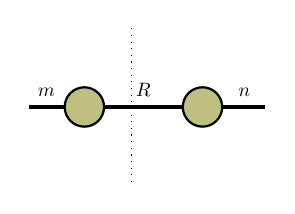
\begin{tikzpicture}[baseline=-0.5ex]
    \tikzset{tensor/.style = {minimum size = 0.5cm,shape = circle,thick,draw=black,inner sep = 0pt}, edge/.style = {thick,line width=.4mm},every loop/.style={}}
    \def\x{6}
    \def\y{0} \node[tensor,fill=green!50!red!50!white] (A) at (\x+1,\y) {$\Ab$};
    \node[tensor,fill=green!50!red!50!white] (B) at (\x+2.5,\y) {$\Bb$};
    \draw[edge] (A) -- (\x+0.3,0) node [midway,above] {\scalebox{0.7}{\dimcolor{$m$}}};
    \draw[edge] (A) -- (B)node [above,midway] {\scalebox{0.7}{\dimcolor{$R$}}};;
    \draw[edge] (B) -- (\x+3.3,\y) node [midway,above] {\scalebox{0.7}{\dimcolor{$n$}}};
    \draw[dotted] (\x+1.6,\y+1) -- (\x+1.6,\y-1);
\end{tikzpicture}\right)\leq R.$$

再考虑如下 $d_1\times d_2$ 矩阵的张量网络表示：
$$
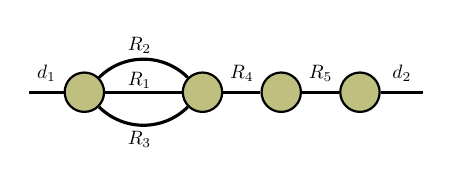
\begin{tikzpicture}[baseline=-0.5ex]
    \tikzset{tensor/.style = {minimum size = 0.5cm,shape = circle,thick,draw=black,inner sep = 0pt}, edge/.style = {thick,line width=.4mm},every loop/.style={}}
    \def\x{6}
    \def\y{0} \node[tensor,fill=green!50!red!50!white] (T) at (\x+1,\y) {$\Tt$};
    \node[tensor,fill=green!50!red!50!white] (A) at (\x+2.5,\y) {$\At$};
    \node[tensor,fill=green!50!red!50!white] (B) at (\x+3.5,\y) {$\Bb$};
      \node[tensor,fill=green!50!red!50!white] (S) at (\x+4.5,\y) {$\Sb$};
    \draw[edge] (T) -- (\x+0.3,\y)node [midway,above] {\scalebox{0.7}{\dimcolor{$d_1$}}};
     \draw[edge] (T) -- (A);
    \draw[edge] (A) -- (B)node [midway,above] {\scalebox{0.7}{\dimcolor{$R_4$}}};
    \draw[edge] (T) to [out=-45,in=-135] (A);
    \draw[edge] (T) to [out=45,in=135] (A);
    \node[draw=none] () at (\x+1.7,\y+0.15) {\scalebox{0.7}{\dimcolor{$R_1$}}};
    \node[draw=none] () at (\x+1.7,\y+0.6) {\scalebox{0.7}{\dimcolor{$R_2$}}};
    \node[draw=none] () at (\x+1.7,\y-0.6) {\scalebox{0.7}{\dimcolor{$R_3$}}};
    \draw[edge](B) -- (S) node [midway,above] {\scalebox{0.7}{\dimcolor{$R_5$}}};
    \draw[edge] (S) -- (\x+5.3,\y) node [midway,above] {\scalebox{0.7}{\dimcolor{$d_2$}}};
    \end{tikzpicture}$$
其中 $\Tt\in\RR^{d_1\times R_1\times R_2\times R_3}$，$\At\in\RR^{R_1\times R_2\times R_3\times R_4}$，$\Bb\in\RR^{R_4\times R_5}$ 且 $\Sb\in\RR^{R_5\times d_2}$。
例如，定理~\ref{thm: matricization-rank} 可用来给出上界
$$
\rank\left(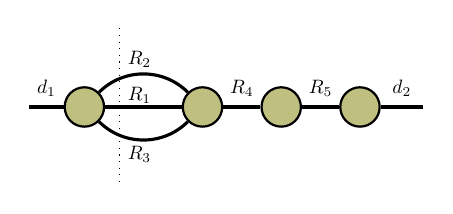
\begin{tikzpicture}[baseline=-0.5ex]
    \tikzset{tensor/.style = {minimum size = 0.5cm,shape = circle,thick,draw=black,inner sep = 0pt}, edge/.style = {thick,line width=.4mm},every loop/.style={}}
    \def\x{6}
    \def\y{0} \node[tensor,fill=green!50!red!50!white] (T) at (\x+1,\y) {$\Tt$};
    \node[tensor,fill=green!50!red!50!white] (A) at (\x+2.5,\y) {$\At$};
    \node[tensor,fill=green!50!red!50!white] (B) at (\x+3.5,\y) {$\Bb$};
      \node[tensor,fill=green!50!red!50!white] (S) at (\x+4.5,\y) {$\Sb$};
    \draw[edge] (T) -- (\x+0.3,\y)node [midway,above] {\scalebox{0.7}{\dimcolor{$d_1$}}};
     \draw[edge] (T) -- (A);
    \draw[edge] (A) -- (B)node [midway,above] {\scalebox{0.7}{\dimcolor{$R_4$}}};
    \draw[edge] (T) to [out=-45,in=-135] (A);
    \draw[edge] (T) to [out=45,in=135] (A);
    \node[draw=none] () at (\x+1.7,\y+0.15) {\scalebox{0.7}{\dimcolor{$R_1$}}};
    \node[draw=none] () at (\x+1.7,\y+0.6) {\scalebox{0.7}{\dimcolor{$R_2$}}};
    \node[draw=none] () at (\x+1.7,\y-0.6) {\scalebox{0.7}{\dimcolor{$R_3$}}};
    \draw[edge](B) -- (S) node [midway,above] {\scalebox{0.7}{\dimcolor{$R_5$}}};
    \draw[edge] (S) -- (\x+5.3,\y) node [midway,above] {\scalebox{0.7}{\dimcolor{$d_2$}}};
    \draw[dotted] (\x+1.45,\y+1) -- (\x+1.45,\y-1);
    \end{tikzpicture}\right)\leq R_1R_2R_3$$
以及
$$
\rank
\left(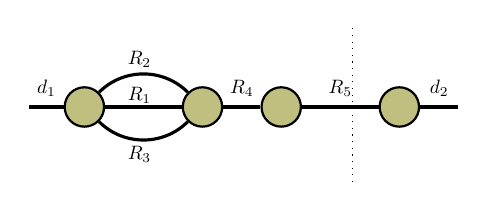
\begin{tikzpicture}[baseline=-0.5ex]
    \tikzset{tensor/.style = {minimum size = 0.5cm,shape = circle,thick,draw=black,inner sep = 0pt}, edge/.style = {thick,line width=.4mm},every loop/.style={}}
    \def\x{6}
    \def\y{0} \node[tensor,fill=green!50!red!50!white] (T) at (\x+1,\y) {$\Tt$};
    \node[tensor,fill=green!50!red!50!white] (A) at (\x+2.5,\y) {$\At$};
    \node[tensor,fill=green!50!red!50!white] (B) at (\x+3.5,\y) {$\Bb$};
      \node[tensor,fill=green!50!red!50!white] (S) at (\x+5,\y) {$\Sb$};
    \draw[edge] (T) -- (\x+0.3,\y)node [midway,above] {\scalebox{0.7}{\dimcolor{$d_1$}}};
     \draw[edge] (T) -- (A);
    \draw[edge] (A) -- (B)node [midway,above] {\scalebox{0.7}{\dimcolor{$R_4$}}};
    \draw[edge] (T) to [out=-45,in=-135] (A);
    \draw[edge] (T) to [out=45,in=135] (A);
    \node[draw=none] () at (\x+1.7,\y+0.15) {\scalebox{0.7}{\dimcolor{$R_1$}}};
    \node[draw=none] () at (\x+1.7,\y+0.6) {\scalebox{0.7}{\dimcolor{$R_2$}}};
    \node[draw=none] () at (\x+1.7,\y-0.6) {\scalebox{0.7}{\dimcolor{$R_3$}}};
    \draw[edge](B) -- (S) node [midway,above] {\scalebox{0.7}{\dimcolor{$R_5$}}};
    \draw[edge] (S) -- (\x+5.75,\y) node [midway,above] {\scalebox{0.7}{\dimcolor{$d_2$}}};
    \draw[dotted] (\x+4.4,\y+1) -- (\x+4.4,\y-1);
    \end{tikzpicture}\right)\leq R_5.
$$
最后一个例子：设 $\Gt\in\RR^{R_1\times\cdots\times R_4}$，$\Ab_1\in\RR^{R_1\times d_1}, \Ab_2\in\RR^{R_2\times d_2},\Ab_3\in\RR^{R_3\times d_3}$ 且 $\Ab_4\in\RR^{R_4\times d_4}$，并考虑张量 $\T = \Gt \times_1 \Ab_1\times_2 \Ab_2\times_3 \Ab_3\times_4 \Ab_4$。定理~\ref{thm: matricization-rank} 例如可用来给出 $\Tt$ 的第一种矩阵化的秩的上界：
$$
\rank(\Tt_{(1)}) = 
\rank\left(
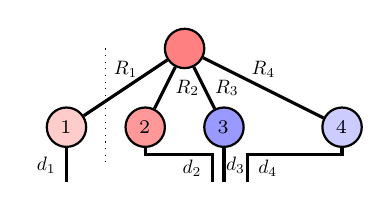
\begin{tikzpicture}[baseline=-0.5ex]
    \tikzset{tensor/.style = {minimum size = 0.5cm,shape = circle,thick,draw=black,inner sep = 0pt}, edge/.style = {thick,line width=.4mm},every loop/.style={}}
    \def\x{6}
    \def\y{0} 
    \node[tensor,fill=red!50!white] (G) at (\x+4.5,\y+1) {$\Gt$};
    \node[tensor,fill=red!20!white] (A_1) at (\x+3,\y){$\Ab_1$};
    \node[tensor,fill=red!40!white] (A_2) at (\x+4,\y){$\Ab_2$};
    \node[tensor, fill=blue!40!white] (A_3) at (\x+5,\y){$\Ab_3$};
    \node[tensor,fill=blue!20!white] (A_4) at (\x+6.5,\y){$\Ab_4$};
    \draw[edge] (G) -- (A_1) node [midway, above] {\scalebox{0.7}{\dimcolor{$R_1$}}};
    \draw[edge] (G) -- (A_2) node [midway, right] {\scalebox{0.7}{\dimcolor{$R_2$}}};
    \draw[edge] (G) -- (A_3) node [midway, right] {\scalebox{0.7}{\dimcolor{$R_3$}}};
    \draw[edge] (G) -- (A_4) node [midway, above] {\scalebox{0.7}{\dimcolor{$R_4$}}};
    \draw[edge] (A_1) -- (\x+3,\y-0.7) node [midway, left] {\scalebox{0.7}{\dimcolor{$d_1$}}};
    \draw[edge] (A_3) -- (\x+5,\y-0.7) node [midway, right=-0.11cm] {\scalebox{0.7}{\dimcolor{$d_3$}}};
    \draw[edge] (A_2) -- (\x+4,\y-0.35) -- (\x+4.85,\y-0.35) -- (\x+4.85,\y-0.7) node [midway, left] {\scalebox{0.7}{\dimcolor{$d_2$}}};
    \draw[edge] (A_4) -- (\x+6.5,\y-0.35) -- (\x+5.30,\y-0.35) -- (\x+5.30,\y-0.7) node [midway, right] {\scalebox{0.7}{\dimcolor{$d_4$}}};
    \draw[dotted](\x+3.5,\y+1)-- (\x+3.5,\y-0.5);
    \end{tikzpicture}\right)\leq R_1.
$$
\paragraph{TN 的边与和式张量。}设 $\T$ 为以 TN 给出的张量。TN 中的任意一条边，都对应一种把该张量表示为若干个与 $\T$ 同尺寸的张量之和的方式。这直接来自 TN 中边的定义。一条边表示一次收缩，而收缩就是一个求和。下面用例子说明这一概念。首先，考虑 $m\times n$ 矩阵的秩为 $R$ 的分解。TN 中的那条边对应把该矩阵表示为 $R$ 个（秩一）矩阵之和：  
$$
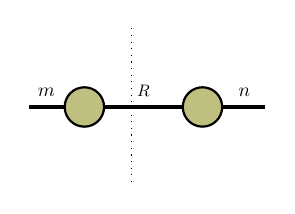
\begin{tikzpicture}[baseline=-0.5ex]
    \tikzset{tensor/.style = {minimum size = 0.5cm,shape = circle,thick,draw=black,inner sep = 0pt}, edge/.style = {thick,line width=.4mm},every loop/.style={}}
    \def\x{6}
    \def\y{0} \node[tensor,fill=green!50!red!50!white] (A) at (\x+1,\y) {$\Ab$};
    \node[tensor,fill=green!50!red!50!white] (B) at (\x+2.5,\y) {$\Bb$};
    \draw[edge] (A) -- (\x+0.3,0) node [midway,above] {\scalebox{0.7}{\dimcolor{$m$}}};
    \draw[edge] (A) -- (B)node [above,midway] {\scalebox{0.6}{\dimcolor{$R$}}};;
    \draw[edge] (B) -- (\x+3.3,\y) node [midway,above] {\scalebox{0.7}{\dimcolor{$n$}}};
    \draw[dotted] (\x+1.6,\y+1) -- (\x+1.6,\y-1);
\end{tikzpicture}
= 
\sum_{r=1}^R
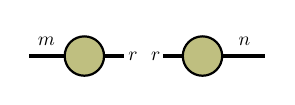
\begin{tikzpicture}[baseline=-0.5ex]
    \tikzset{tensor/.style = {minimum size = 0.5cm,shape = circle,thick,draw=black,inner sep = 0pt}, edge/.style = {thick,line width=.4mm},every loop/.style={}}
    \def\x{6}
    \def\y{0} \node[tensor,fill=green!50!red!50!white] (A) at (\x+1,\y) {$\Ab$};
    \node[tensor,fill=green!50!red!50!white] (B) at (\x+2.5,\y) {$\Bb$};
    \draw[edge] (A) -- (\x+0.3,0) node [midway,above] {\scalebox{0.7}{\dimcolor{$m$}}};
    \draw[edge] (A) -- (\x+1.5,\y) node [pos=1.5] {\scalebox{0.7}{\indcolor{$r$}}};
    \draw[edge] (B) -- (\x+3.3,\y) node [midway,above] {\scalebox{0.7}{\dimcolor{$n$}}};
    \draw[edge](B) -- (\x+2,\y)node [pos=1.4] {\scalebox{0.7}{\indcolor{$r$}}};
\end{tikzpicture}
= \sum_{r=1}^R \Ab_{:,r} \Bb_{r,:} = \sum_{r=1}^R \ab_r \outprod \bb_r,
$$
其中 $\ab_r$ 为 $\Ab\in\RR^{m\times R}$ 的各列，$\bb_r$ 为 $\Bb\in\RR^{R\times n}$ 的各行。

